\documentclass[11pt,a4paper]{article}
\usepackage[utf8]{inputenc}
%\usepackage[german]{babel}
\usepackage[T1]{fontenc}
\usepackage{amsmath}
\usepackage{amsfonts}
\usepackage{amssymb}
\usepackage{listings}
\lstset{
numbers=left, 
numberstyle=\small, 
numbersep=8pt, 
frame = single, 
%language=Pascal, 
framexleftmargin=15pt}
\usepackage{graphicx}
\usepackage{fourier}
\usepackage[left=2cm,right=2cm,top=2cm,bottom=2cm]{geometry}




\begin{document}
\section{Mobile phones and Radio cells}
\subsection{Radio cells}
Radio cells are necessary to connect with mobile phones, in particular with the SIM card, and provide access to the telecommunication network. If a SIM card is in reach (the sending radius) of the radio cell, it will be appended to the radio cell's list of near mobile phones. That way, we can deduce, that the SIM has to be inside the radius and we can constrain the phone's location to the inside of the circle around the radio cell's location.

Here, another important constrain can be made, when other radio cells are also detecting the same SIM at the same time. We can reduce the intersecting area of the sending radii as the possible area where the SIM is located. 
This will be important for the reverse settings (section \ref{sec:reverse}), since we can set the agents of interest to this location and animate possible behaviour.

\subsection{Intersection}
To compute the intersection I wrote the folling script:

\begin{lstlisting}[language = Python, caption={Intersection of circles}]
def pointsInCircle(r, xm, ym ):
    
    xmin = xm - r
    xmax = xm + r
    ymin = ym - r
    ymax = ym + r
    
    xs = range(xmin, xmax+1)
    ys = range(ymin, ymax+1)
    print("Points in circle (",r,xm, ym,") :")
    pic = set() # set of points in circle
    for x in xs:
        for y in ys:
            if (x-xm)**2 + (y-ym)**2 <= r**2:
                pic.add((x,y))
    print(pic)
    return pic
                       
pic1 = pointsInCircle(3, 1, 2)        
pic2 = pointsInCircle(2, 3, 2) 
intersection = pic1.intersection(pic2)   
print("intersect: ", intersection)
\end{lstlisting}

\section{Reverse settings}
\label{sec:reverse}
After running a simulation, we obtain a partial dataset of the agents and their actions. The goal is to create possible ways of what might have happened. In that sense we use the data and  the deductions made from it to create a new setting of a simulation ( or only of an animation, in which all actions are clearly defined ).

\section{Settings}
\subsection{bpy module}
There are a couple of possibilities to startup a simulation. I suggest to use the \texttt{bpy} module for setting all agents and artefacts, including all dependencies, like possession of things. These include e.g. mobile phones, cars, keys, bankcards \dots

The \texttt{bpy} module supports reading text files, so that one can create an external configuration file of a priori known data ( like names, birthdate, home, bankcard, car, friends, relationships \dots)

\begin{lstlisting}[language = Python, caption={Example config file to set personalities. Here the textfile uses already Python syntax for Python dictionaries.}]
{'surname':'Thomas','name':'Meyer', 'age':28, 'mobilePhone':78,'bankcard':'300112'}
{'surname':'Anna','name':'Xing', 'age':42, 'mobilePhone':2}
{'surname':'Lucas','name':'Guterres', 'age':56, 'mobilePhone':31}
\end{lstlisting}

For getting such data into Blender one can use a script like the following. Since it is already in Python syntax, I use the \texttt{eval()} method. For future work it might be better to use XML format for the configuration files and adapt the import scripts to it.

\begin{lstlisting}[language = Python, caption=Excerpt from \textit{setPersonalities.py} in \textit{setups\_2021\_09\_07.blend}, label=setPersons]
import bpy
dicts = []
path = "/home/.../configuration.txt"

with open(path,"r") as f:
    lines = f.read().splitlines()    
for l in lines: 
    dicts.append(eval(l)) 
    
# entry of persons database == each is one dictionary    
for entry in range(len(lines)):    
    bpy.ops.mesh.primitive_uv_sphere_add(size=1, location=(0+2*entry, 0, 1)) 
    ob = bpy.context.object
    ob.name = ( dicts[entry]['surname'] + " " + dicts[entry]['name'] )
    ob.show_name = True  
    for attr in dicts[entry]:
        # create attributes from config file
        ob[attr] = dicts[entry][attr]   
    if 'mobilePhone' in ob:
        bpy.ops.mesh.primitive_cube_add(radius=0.3, location=(0, 0, 2.5) )
        ob_c = bpy.context.object  # will be child (c) object  
        ob_c.name = ( "MobilePhone " + str(dicts[entry]['mobilePhone']) )        
\end{lstlisting}

The new agents are set into the scene according to the location attribute ( which is here just aligned to each other). 
\begin{figure}
\centering
%\begin{tabular}{cc}
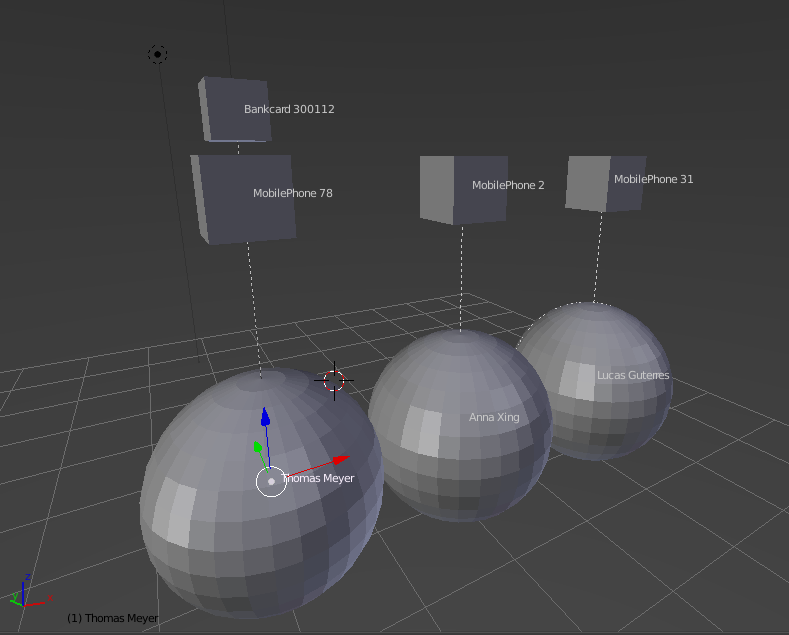
\includegraphics[scale=0.45]{../Pictures/create_agents.png} % &
%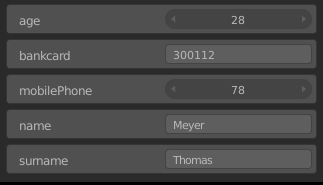
\includegraphics[scale=0.4]{../Pictures/properties_agents.png}
%\end{tabular}
\caption{After running the \textit{setPersonalities.py} script in setups\_2021\_09\_05.blend The agents are represented as simple spheres. Items like mobile phones or cards are cube-shaped and white dashed lines represent parentship.}
\end{figure}
 
The simulation is not started yet.

\subsection{bge module}
As soon the simulaton is running, the \textit{bge module} is accessible. Since the game engine normally reads the scripts every single frame, we also have to create a startup script inside the simulation, which is only executed once at the very first frame of the simulation. I use this to read the properties of the agents and artefacts that were set befor via the configuration file and the bpy module. In the course of this reading, the properties are passed to the corresponding \textit{game properties}. (Note that game properties are not available before the game engine was started.) 

\section{Time schedules}
\subsection{Everyday life}
Instead of randomly acting agents, there should also be the possibility to assign structured time schedules to agents. This will include \\

\begin{minipage}{0.4\textwidth}
\begin{itemize}
\item wake up at home
\item go to work / school
\item work 
\item come home again
\item visit friends
\item go to cinema/ theatre/ fitness
\item come home again
\item sleep
\end{itemize}
and many more. 
\end{minipage} \hfill\begin{minipage}{0.55\textwidth}
\begin{lstlisting}[language = Python, breaklines=true,  caption={Basic time structure for normal agent's day}]
import bpy
# time values  
base = [ 40, 130, 240, 350, 400, 430, 600 ]  
var = 15   # variance
day = [ x + rd.randint(-var, var) for x in base ]
day.sort()
\end{lstlisting}
\end{minipage}\\
The structure should be satisfiable, meaning that times and distances are in realstic proportion to each other - so that a target can be reached in reasonable time.

\subsection{Quasi Random Walkers}
Depending on the simulation there could also be the need for quasi-randomly walking agents. One way to do this is to choose a random number of targets ( on the navigation mesh ) and then assign randomly time values to the targets. It's essential to use the \texttt{sort()} method. The created lists are passed to the walkers' properties.
\begin{lstlisting}[language = Python, breaklines=true, caption={randomWalkers}]
for obj in sce.objects:
                                                                            
    if "rWalker_" in obj.name: 
        targets = rd.choices(meshes, k=rd.randint(5, 15))
        times = rd.sample(range(1, 100), len(targets)) 
        times.sort()           
        obj['targets'] = targets
        obj['day'] = times 
\end{lstlisting}        
The difference to \textit{Everyday life} agents is, that here is no assurance that the agents will reach their goal and that the walking behaviour would be very realistic.

\subsection{Explicitly timed agents} 
These agents have a detailed ``story''.

\section{GIS}
\subsection{Satellite basemap}
For getting a better feeling of the scene of interest it is possible to import the satellite basemap. I created one for Potsdam, Luisenplatz, and one for Genova, Porto Antico. It helps to get an idea of possible artefacts, like cars and trees.\\
\begin{figure}
\begin{tabular}{ccc}
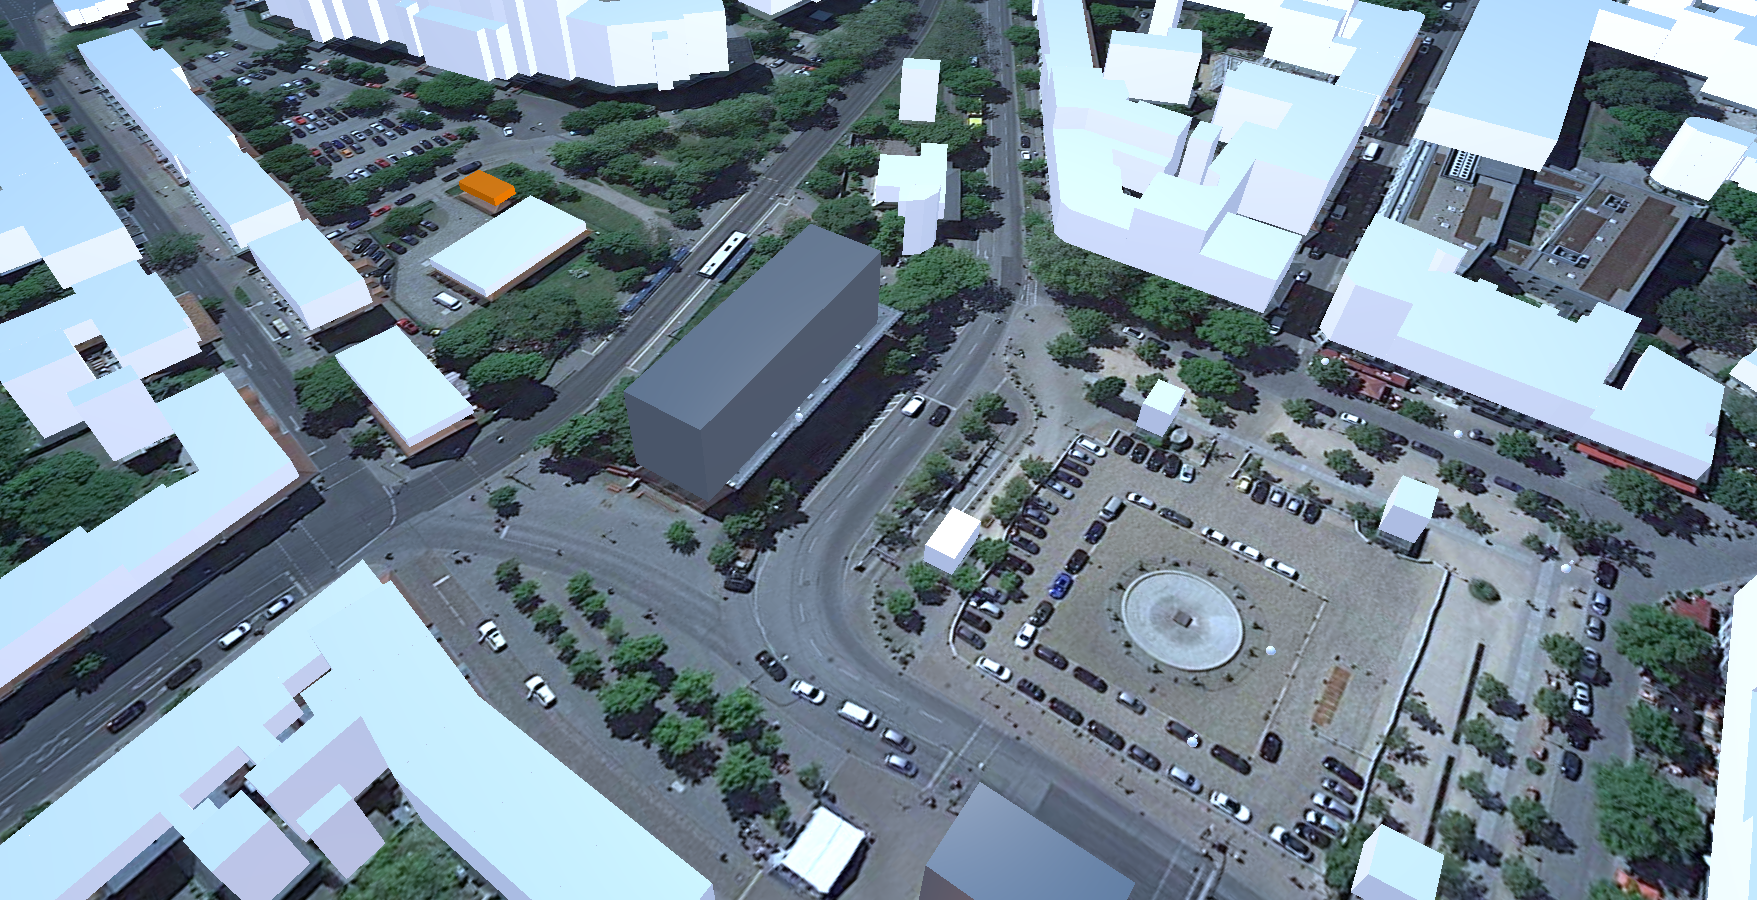
\includegraphics[width=0.45\textwidth]{../Pictures/luisenplatz_sat.png} &
\ \hfill &
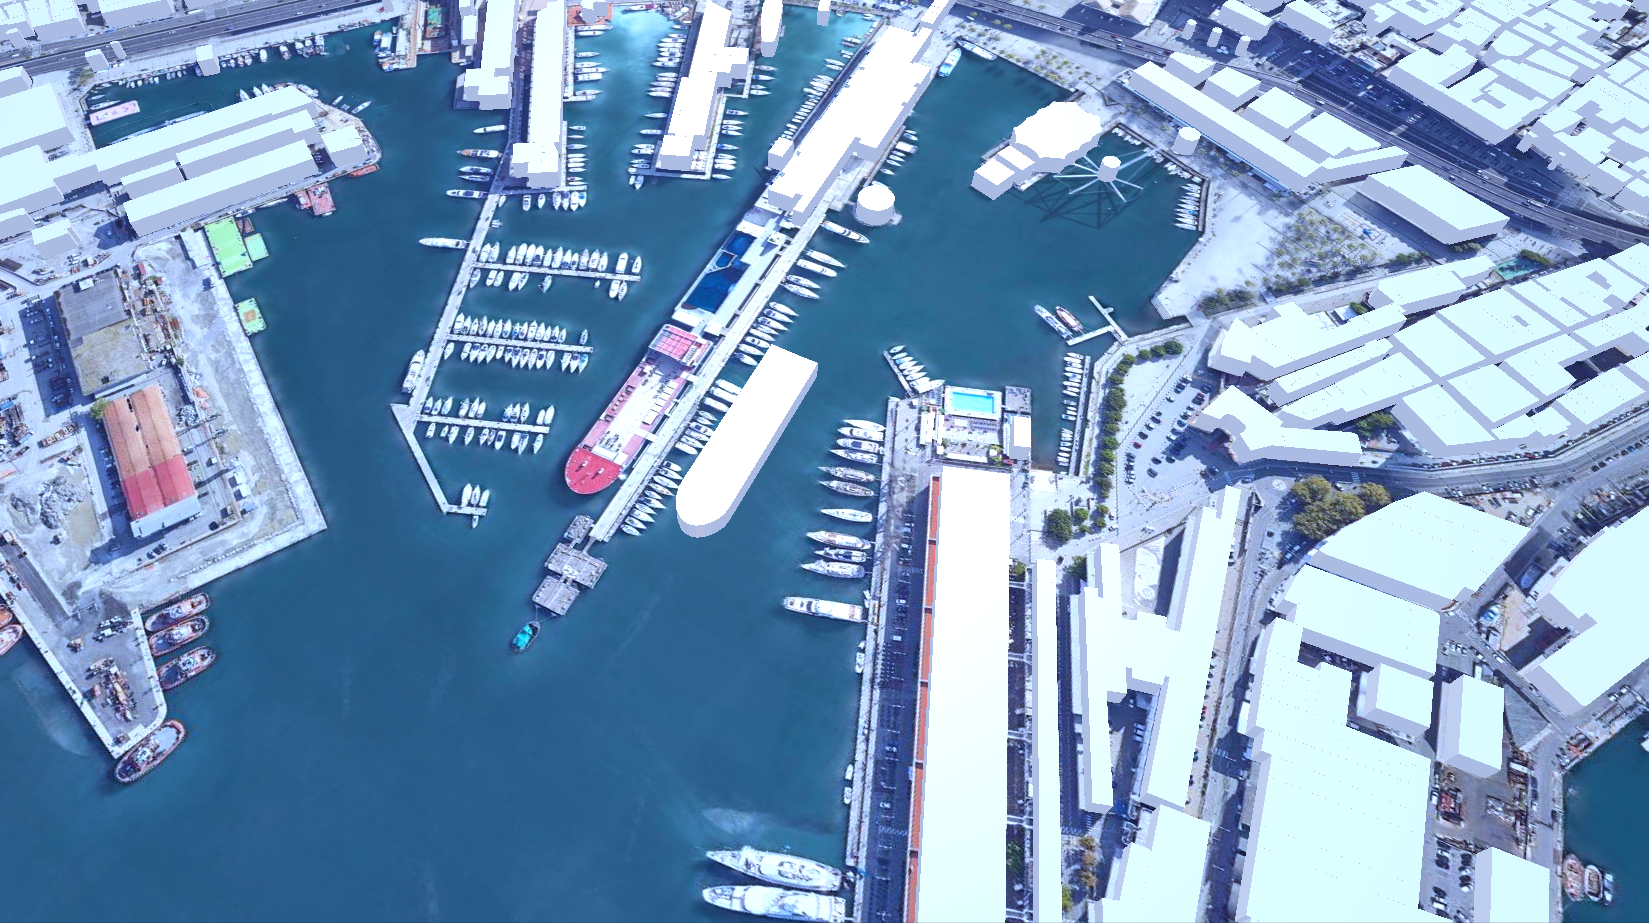
\includegraphics[width=0.42\textwidth]{../Pictures/portoantico.png}
\end{tabular}
\caption{Using satellite basemap for two exemplary scenarios. \textit{Left:} Luisenplatz, Potsdam. \textit{Right:} Porto Antico, Genova}
\end{figure}
 
\subsection{Dimensions}
The BlenderGIS addon adjusts the Blender scene to the right dimensions. In the scene options I choose the metric system. Therefore, one \textit{Blender units} equals one meter and the geographic data are congruent with this unit system. 
Having this realistic makes it easier to use as velocity measure SI-units, i.e. m/s. \footnote{As long time scale of the simulation is set to 1. }

\section{Time}
We want to represent time as integers, because \textit{clingo} needs to. Moreover, an integer representation is easier to read. There is one script I call \textit{universalTime.py} that gets the game engine time and cuts it down using the \texttt{floor()} function of the \texttt{math} module. 
\begin{lstlisting}[language = Python, breaklines=true, caption={Universal Time}]
time_scale = 1 # x-fache Geschwindigkeit    
bge.logic.setTimeScale(time_scale)
t = bge.logic.getClockTime()

own["intTime_old"] = own["intTime"] 
own["intTime"] = m.floor(t)         
diff = own["intTime_old"] - own["intTime"] 
own['diff'] = diff
  
if diff != 0:
    print(own["intTime"] ) 
\end{lstlisting}
In line 11 the script prints the integer time to the console. I use the auxiliary property `diff' to make sure that the floored time value is only printed once instead of multiple times the same integer. That way the console prints every integer time step, which makes it convenient to monitor what's going on in the running simulation.



\section{Output Log-files}
\subsection{A priori facts}
The first output files are going to be produced already before the simulation starts. In fact, it's more a question of how to look on it, because the only difference to a configuration file would be the syntax used. But here I assume, that the output file will be something that \textit{clingo} understands. 
For example, while setting up the scene we can write all facts that are a priori known to a file like \texttt{initial\_facts.lp}. 
\begin{lstlisting}[caption={A priori facts for clingo}]
radioCell( "Radio Cell.002", loc(-612,-447), radius(1400) ).
radioCell( "Radio Cell.001", loc(395,-267), radius(300) ).
radioCell( "Radio Cell", loc(-219,244), radius(200) ).
\end{lstlisting}
In this case we receive the facts about three radio cells, including their name (as a string), location (in meters) and their sending radius. We can extend this knowledge base with persons and their possessions etc.

\subsection{Runtime facts}
Those are the facts that will be produced during the simulatio is running.
Maybe also here one could consider to use XML format as intermediate step for future projects. For now, I'm writing the information from the settings and the simulation directly to textfiles in \textit{clingo} syntax. 
\begin{lstlisting}[language = Python, breaklines=true, caption={Log-file thief}]
own = cont.owner
t = str(intTime)
x = str(m.floor(own.worldPosition.x))
y = str(m.floor(own.worldPosition.y))

with open(str(own.name)+"_log.lp", "a") as f:
    f.write( 'at( "'+str(own)+'", loc('+x+','+y+'), '+t+' )'+"\n" )  
    f.write( 'stole( ' + 'mphone( mobile_phone_2 '+')'+', '+'loc('+x+','+y+')'+', '+ t +')'+'.' +"\n" ) 
    
if diff != 0:
    with open(str(own.name)+"_log.lp", "a") as f:
        f.write( 'at( "'+str(own)+'", loc('+x+','+y+'), '+t+' ).'+"\n" )    
\end{lstlisting}
In line 10 we use again the `diff' property to print only one line per agent and time step. 

(By the way, here is a problem that is yet to be solved: in line 6 the script outputs the moment of the theft as the usual \texttt{at(P,L,T)} predicate/atom. Since the time is cut down to the integer value there can be two different values for the location at the same integer time point. I could ignore one of it - but maybe its useful to track the float time and receive a higher time resolution for later use\dots)

Another example: again facts regarding radio cells being created.
\begin{lstlisting}[language = Python, breaklines=true, caption={Log-file radio cell}]
for mph in own['mobilePhones']:
    if (own.worldPosition - mph.worldPosition).length < own['radius'] and not own in mph["radioCells"]:
        mph["radioCells"].append(own)
        with open("radioCells_log.lp", "a") as f:
            f.write( 'available( "'+own.name+'", "'+mph.name+'", '+str(intTime)+' ).')
        
    if (own.worldPosition - mph.worldPosition).length >= own['radius'] and own in mph["radioCells"]:
        mph["radioCells"].remove(own)
        with open("radioCells_log.lp", "a") as f:
            f.write( 'unavailable( "'+own.name+'", "'+mph.name+'", '+str(intTime)+' ).')
\end{lstlisting}
That script yields facts like
\begin{lstlisting}
available( "Radio Cell.002", "MobilePhone 31", 0 ).
available( "Radio Cell.001", "MobilePhone 78", 0 ).
available( "Radio Cell", "MobilePhone 31", 0 ).
available( "Radio Cell", "MobilePhone 78", 0 ).
unavailable( "Radio Cell", "MobilePhone 78", 18 ).
\end{lstlisting}
depending on how the \textit{mobile phones} are moving through the scene.\footnote{I emphasized mobile phone to make clear that this does not automatically mean that also the owner is moving. Also, it should be the SIM card, not the mobile phone, being precise.} 
Let's track a simple moving person, Lucas Guterres.

\begin{lstlisting}
at( "Lucas Guterres", loc(-98,154), 1 ).
at( "Lucas Guterres", loc(-98,154), 2 ).
at( "Lucas Guterres", loc(-98,154), 3 ).
at( "Lucas Guterres", loc(-98,154), 4 ).
at( "Lucas Guterres", loc(-98,154), 5 ).
at( "Lucas Guterres", loc(-82,140), 6 ).
at( "Lucas Guterres", loc(-66,126), 7 ).
at( "Lucas Guterres", loc(-50,112), 8 ).
at( "Lucas Guterres", loc(-34,98), 9 ).
at( "Lucas Guterres", loc(-18,84), 10 ).
\end{lstlisting}

\section{Reasoning}
If we continue with the last tracked facts of Lucas Guterres we can build a first theory. E.g. in the first time steps there's always the same location - for the moment one time step means one second. At least when regarding this time resolution we can deduce that Lucas isn't moving.
Not moving might be called \textit{staying}.
\begin{lstlisting}[breaklines=true, numbers=none]
{ staying( T, T'-T, loc(X,Y), P ) ; unknown_path( T, T'-T, P) } = 1 
	:- at( P, loc(X,Y), T ), at( P, loc(X,Y), T'), T<T' .
\end{lstlisting}
The alternative in the choice rule is \textit{unknown\_path}. The idea is, that if a time interval is greater without knowledge of the agent's or artefact's location, we have to deal with the possibility that the agent was not staying but moved away and returned to the starting point.
Two different answer sets will be computed. 
If we assume that the agent did not stay, we can assume movement.
\begin{lstlisting}[breaklines=true, numbers=none]
moved( P, loc(X,Y), loc(X',Y'), T, T'-T ) 
	:- at( P, loc(X',Y'), T' ), at( P, loc(X,Y), T), T'>T, loc(X',Y')!=loc(X,Y), not staying( T, _, _, P).
\end{lstlisting}
\subsection{External calculation with Python}
For reconstructing the velocity of a person it would be handy to have the euclidian distance. Therefore, I use an external Python function which returns the distance to an atom \texttt{dist\_eukl()}

\begin{lstlisting}
#script (python)

import clingo
import math

N = clingo.Number
def dist(x, y):
    xn = x.number
    yn = y.number
    d = math.sqrt(xn**2 + yn**2)
    d_int = math.floor(d)
    return N(d_int)

#end.

%% Manhattan distance
dist_manh( |X-X'|, |Y-Y'|, loc(X,Y), loc(X',Y') )   
	:- moved( P, loc(X,Y), loc(X',Y'), _, _ ).
%% Euclidian distance	      
dist_eukl( @dist(Xm,Ym), loc(X,Y), loc(X',Y') )    
	:- dist_manh( Xm,Ym, loc(X,Y), loc(X',Y')).    
\end{lstlisting}

For calculating the velocity I used again a Python function ( probably works also directly in clingo ), by deviding the euclidian distance by the time interval.
\begin{lstlisting}[numbers=none]
speed( P, T, T'-T, D, @div(D,T'-T) ) 
	:-  moved( P, loc(X,Y), loc(X',Y'), T, T'-T ),
	 dist_eukl( D, loc(X,Y), loc(X',Y') ), time(T), time(T').
\end{lstlisting}	 
Comparing the results with the actual velocity inside the simulation shows high accordance.





\section{Inside buildings}
\lstlistoflistings




       
\end{document}
